\documentclass[10pt]{article}

\usepackage[margin=1in]{geometry}
\usepackage{amsmath}
\usepackage{amssymb}
\usepackage{amsthm}
\usepackage{mathtools}
\usepackage[shortlabels]{enumitem}
\usepackage[normalem]{ulem}
\usepackage{courier}
\usepackage[T1]{fontenc}
\usepackage{upquote}

\usepackage{hyperref}
\hypersetup{
  colorlinks   = true, %Colours links instead of ugly boxes
  urlcolor     = black, %Colour for external hyperlinks
  linkcolor    = blue, %Colour of internal links
  citecolor    = blue  %Colour of citations
}

\usepackage{accsupp}
\newcommand{\noncopynumber}[1]{%
    \BeginAccSupp{method=escape,ActualText={}}#1\EndAccSupp{}%
}
\usepackage{listings}
\lstset{
    language=HTML
    ,basicstyle=\linespread{1}\ttfamily
    ,keywordstyle=
    ,language=sh
    ,showstringspaces=false
    ,numbers=left
    ,breaklines=false
    ,numbers=left
    ,numberstyle=\tiny\noncopynumber
    }

\usepackage{array}
\newcolumntype{L}[1]{>{\raggedright\arraybackslash}p{#1}}


%%%%%%%%%%%%%%%%%%%%%%%%%%%%%%%%%%%%%%%%%%%%%%%%%%%%%%%%%%%%%%%%%%%%%%%%%%%%%%%%

\theoremstyle{definition}
\newtheorem{problem}{Problem}
\newtheorem{note}{Note}
\newcommand{\E}{\mathbb E}
\newcommand{\R}{\mathbb R}
\DeclareMathOperator{\Var}{Var}
\DeclareMathOperator*{\argmin}{arg\,min}
\DeclareMathOperator*{\argmax}{arg\,max}

\newcommand{\trans}[1]{{#1}^{T}}
\newcommand{\loss}{\ell}
\newcommand{\w}{\mathbf w}
\newcommand{\mle}[1]{\hat{#1}_{\textit{mle}}}
\newcommand{\map}[1]{\hat{#1}_{\textit{map}}}
\newcommand{\normal}{\mathcal{N}}
\newcommand{\x}{\mathbf x}
\newcommand{\y}{\mathbf y}
\newcommand{\ltwo}[1]{\lVert {#1} \rVert}

%%%%%%%%%%%%%%%%%%%%%%%%%%%%%%%%%%%%%%%%%%%%%%%%%%%%%%%%%%%%%%%%%%%%%%%%%%%%%%%%

\begin{document}
\begin{center}
{
\Large
Quiz Practice: POSIX Shell 1
}
\vspace{0.1in}
\end{center}

\begin{note}
    I will generate new problems by:
    (1) changing the type of quotation mark,
    (2) removing/adding quotation marks.
\end{note}

\noindent\vspace{0.1in}\begin{minipage}{\textwidth}
\section{Glob}

\begin{note}
The POSIX shell has a built-in pattern matching feature for working with files.
The glob operator \lstinline{*} matches zero or more of any character,
and the question operator \lstinline{?} matches exactly one of any character.
The \lstinline{*} and \lstinline{?} operators do not match a dot at the beginning of the file, and so do not match hidden files.


\end{note}

\end{minipage}
\noindent\vspace{0.1in}\begin{minipage}{\textwidth}

\begin{problem}
Write the output of the final command in the following terminal session.
Do not provide any additional information,
such as explanations.
If the command has no output,
then do not write anything.

\end{problem}
\begin{lstlisting}
$ cd; rm -rf quiz; mkdir quiz; cd quiz
$ touch hello world
$ touch hola mundo 
$ touch salve munde
$ rm *e*
$ ls | wc -l
\end{lstlisting}

Fraction of LLMs with correct answer: 5 / 22 = 0.23
\end{minipage}
\noindent\vspace{0.1in}\begin{minipage}{\textwidth}

\begin{problem}
Write the output of the final command in the following terminal session.
Do not provide any additional information,
such as explanations.
If the command has no output,
then do not write anything.

\end{problem}
\begin{lstlisting}
$ cd; rm -rf quiz; mkdir quiz; cd quiz
$ touch hello world
$ touch hola mundo 
$ touch salve munde
$ rm e*
$ ls | wc -l
\end{lstlisting}

Fraction of LLMs with correct answer: 3 / 21 = 0.14
\end{minipage}
\noindent\vspace{0.1in}\begin{minipage}{\textwidth}

\begin{problem}
Write the output of the final command in the following terminal session.
Do not provide any additional information,
such as explanations.
If the command has no output,
then do not write anything.

\end{problem}
\begin{lstlisting}
$ cd; rm -rf quiz; mkdir quiz; cd quiz
$ touch hello world
$ touch hola mundo 
$ touch salve munde
$ rm *e
$ ls | wc -l
\end{lstlisting}

Fraction of LLMs with correct answer: 3 / 20 = 0.15
\end{minipage}
\noindent\vspace{0.1in}\begin{minipage}{\textwidth}

\begin{problem}
Write the output of the final command in the following terminal session.
Do not provide any additional information,
such as explanations.
If the command has no output,
then do not write anything.

\end{problem}
\begin{lstlisting}
$ cd; rm -rf quiz; mkdir quiz; cd quiz
$ touch .hello world
$ touch .hola mundo 
$ touch .salve munde
$ rm *e*
$ ls -a | wc -l
\end{lstlisting}

Fraction of LLMs with correct answer: 3 / 19 = 0.16
\end{minipage}
\noindent\vspace{0.1in}\begin{minipage}{\textwidth}

\begin{problem}
Write the output of the final command in the following terminal session.
Do not provide any additional information,
such as explanations.
If the command has no output,
then do not write anything.

\end{problem}
\begin{lstlisting}
$ cd; rm -rf quiz; mkdir quiz; cd quiz
$ touch .hello world
$ touch .hola mundo 
$ touch .salve munde
$ rm .*e
$ ls -a | wc -l
\end{lstlisting}

Fraction of LLMs with correct answer: 2 / 19 = 0.11
\end{minipage}
\noindent\vspace{0.1in}\begin{minipage}{\textwidth}

\begin{problem}
Write the output of the final command in the following terminal session.
Do not provide any additional information,
such as explanations.
If the command has no output,
then do not write anything.

\end{problem}
\begin{lstlisting}
$ cd; rm -rf quiz; mkdir quiz; cd quiz
$ touch "hello world"
$ touch "hola mundo"
$ touch "salve munde"
$ rm *d?
$ ls | wc -l
\end{lstlisting}

Fraction of LLMs with correct answer: 5 / 19 = 0.26
\end{minipage}
\noindent\vspace{0.1in}\begin{minipage}{\textwidth}

\begin{problem}
Write the output of the final command in the following terminal session.
Do not provide any additional information,
such as explanations.
If the command has no output,
then do not write anything.

\end{problem}
\begin{lstlisting}
$ cd; rm -rf quiz; mkdir quiz; cd quiz
$ touch "hello world"
$ touch "hola mundo"
$ touch "salve munde"
$ rm *d?
$ ls | wc -l
\end{lstlisting}

Fraction of LLMs with correct answer: 5 / 19 = 0.26
\end{minipage}
\noindent\vspace{0.1in}\begin{minipage}{\textwidth}
\subsection{Weirdness}

\begin{note}
The glob does not expand within quotes.
If the glob expression has no matches,
then the literal expression is passed as an argument.

\end{note}

\end{minipage}
\noindent\vspace{0.1in}\begin{minipage}{\textwidth}

\begin{problem}
Write the output of the final command in the following terminal session.
Do not provide any additional information,
such as explanations.
If the command has no output,
then do not write anything.

\end{problem}
\begin{lstlisting}
$ cd; rm -rf quiz; mkdir quiz; cd quiz
$ touch "hello world"
$ touch "hola mundo"
$ touch "salve munde"
$ touch *
$ ls | wc -l
\end{lstlisting}

Fraction of LLMs with correct answer: 4 / 19 = 0.21
\end{minipage}
\noindent\vspace{0.1in}\begin{minipage}{\textwidth}

\begin{problem}
Write the output of the final command in the following terminal session.
Do not provide any additional information,
such as explanations.
If the command has no output,
then do not write anything.

\end{problem}
\begin{lstlisting}
$ cd; rm -rf quiz; mkdir quiz; cd quiz
$ touch *
$ ls | wc -l
\end{lstlisting}

Fraction of LLMs with correct answer: 4 / 19 = 0.21
\end{minipage}
\noindent\vspace{0.1in}\begin{minipage}{\textwidth}

\begin{problem}
Write the output of the final command in the following terminal session.
Do not provide any additional information,
such as explanations.
If the command has no output,
then do not write anything.

\end{problem}
\begin{lstlisting}
$ cd; rm -rf quiz; mkdir quiz; cd quiz
$ touch *
$ ls | wc -l
\end{lstlisting}

Fraction of LLMs with correct answer: 4 / 19 = 0.21
\end{minipage}
\noindent\vspace{0.1in}\begin{minipage}{\textwidth}

\begin{problem}
Write the output of the final command in the following terminal session.
Do not provide any additional information,
such as explanations.
If the command has no output,
then do not write anything.

\end{problem}
\begin{lstlisting}
$ cd; rm -rf quiz; mkdir quiz; cd quiz
$ touch "hello world"
$ touch "hola mundo"
$ touch "salve munde"
$ touch "*"
$ ls | wc -l
\end{lstlisting}

Fraction of LLMs with correct answer: 13 / 19 = 0.68
\end{minipage}
\noindent\vspace{0.1in}\begin{minipage}{\textwidth}

\begin{problem}
Write the output of the final command in the following terminal session.
Do not provide any additional information,
such as explanations.
If the command has no output,
then do not write anything.

\end{problem}
\begin{lstlisting}
$ cd; rm -rf quiz; mkdir quiz; cd quiz
$ touch "hello world"
$ touch "hola mundo"
$ touch "salve munde"
$ touch "*"
$ ls | wc -l
\end{lstlisting}

Fraction of LLMs with correct answer: 12 / 19 = 0.63
\end{minipage}
\noindent\vspace{0.1in}\begin{minipage}{\textwidth}
\subsection{For Loops}

\begin{note}
Glob expansion happens after the shell processes the spaces that separate the list of strings to loop over.

\end{note}

\end{minipage}
\noindent\vspace{0.1in}\begin{minipage}{\textwidth}

\begin{problem}
Write the output of the final command in the following terminal session.
Do not provide any additional information,
such as explanations.
If the command has no output,
then do not write anything.

\end{problem}
\begin{lstlisting}
$ cd; rm -rf quiz; mkdir quiz; cd quiz
$ touch "hello world"
$ touch "hola mundo"
$ touch "salve munde"
$ for i in *; do echo $i; done | wc -l
\end{lstlisting}

Fraction of LLMs with correct answer: 14 / 19 = 0.74
\end{minipage}
\noindent\vspace{0.1in}\begin{minipage}{\textwidth}

\begin{problem}
Write the output of the final command in the following terminal session.
Do not provide any additional information,
such as explanations.
If the command has no output,
then do not write anything.

\end{problem}
\begin{lstlisting}
$ cd; rm -rf quiz; mkdir quiz; cd quiz
$ touch hello world
$ touch hola mundo
$ touch salve munde
$ for i in *; do echo $i; done | wc -l
\end{lstlisting}

Fraction of LLMs with correct answer: 7 / 19 = 0.37
\end{minipage}
\noindent\vspace{0.1in}\begin{minipage}{\textwidth}

\begin{problem}
Write the output of the final command in the following terminal session.
Do not provide any additional information,
such as explanations.
If the command has no output,
then do not write anything.

\end{problem}
\begin{lstlisting}
$ cd; rm -rf quiz; mkdir quiz; cd quiz
$ touch hello world
$ touch hola mundo
$ touch salve munde
$ for i in "*"; do echo $i; done | wc -l
\end{lstlisting}

Fraction of LLMs with correct answer: 5 / 19 = 0.26
\end{minipage}
\noindent\vspace{0.1in}\begin{minipage}{\textwidth}

\begin{problem}
Write the output of the final command in the following terminal session.
Do not provide any additional information,
such as explanations.
If the command has no output,
then do not write anything.

\end{problem}
\begin{lstlisting}
$ cd; rm -rf quiz; mkdir quiz; cd quiz
$ for i in *; do echo $i; done | wc -l
\end{lstlisting}

Fraction of LLMs with correct answer: 3 / 19 = 0.16
\end{minipage}
\noindent\vspace{0.1in}\begin{minipage}{\textwidth}
\subsection{Security}

\begin{note}
Glob expansion happens in the shell,
before the parameters are sent to the program.
This can have unintended side effects.
If you are working in a directory where someone else is allowed to create files,
they can create files that will be expanded by \lstinline{*} into command line arguments.
This problem can be mitigated by using \lstinline{./*} instead of \lstinline{*}.
Command line arguments that appear after a \lstinline{--} will never be interpreted as command line arguments.

\end{note}

\end{minipage}
\noindent\vspace{0.1in}\begin{minipage}{\textwidth}

\begin{problem}
Write the output of the final command in the following terminal session.
Do not provide any additional information,
such as explanations.
If the command has no output,
then do not write anything.

\end{problem}
\begin{lstlisting}
$ cd; rm -rf quiz; mkdir quiz; cd quiz
$ mkdir test
$ rm *
$ ls
\end{lstlisting}

Fraction of LLMs with correct answer: 9 / 19 = 0.47
\end{minipage}
\noindent\vspace{0.1in}\begin{minipage}{\textwidth}

\begin{problem}
Write the output of the final command in the following terminal session.
Do not provide any additional information,
such as explanations.
If the command has no output,
then do not write anything.

\end{problem}
\begin{lstlisting}
$ cd; rm -rf quiz; mkdir quiz; cd quiz
$ mkdir test
$ echo evil > -rf
$ rm *
$ ls
\end{lstlisting}

Fraction of LLMs with correct answer: 7 / 19 = 0.37
\end{minipage}
\noindent\vspace{0.1in}\begin{minipage}{\textwidth}

\begin{problem}
Write the output of the final command in the following terminal session.
Do not provide any additional information,
such as explanations.
If the command has no output,
then do not write anything.

\end{problem}
\begin{lstlisting}
$ cd; rm -rf quiz; mkdir quiz; cd quiz
$ mkdir test
$ echo evil > -rf
$ rm ./*
$ ls
\end{lstlisting}

Fraction of LLMs with correct answer: 8 / 19 = 0.42
\end{minipage}
\noindent\vspace{0.1in}\begin{minipage}{\textwidth}

\begin{problem}
Write the output of the final command in the following terminal session.
Do not provide any additional information,
such as explanations.
If the command has no output,
then do not write anything.

\end{problem}
\begin{lstlisting}
$ cd; rm -rf quiz; mkdir quiz; cd quiz
$ mkdir test
$ rm -- -rf *
$ ls
\end{lstlisting}

Fraction of LLMs with correct answer: 15 / 19 = 0.79
\end{minipage}
\noindent\vspace{0.1in}\begin{minipage}{\textwidth}

\begin{problem}
Write the output of the final command in the following terminal session.
Do not provide any additional information,
such as explanations.
If the command has no output,
then do not write anything.

\end{problem}
\begin{lstlisting}
$ cd; rm -rf quiz; mkdir quiz; cd quiz
$ mkdir test
$ rm -rf -- *
$ ls
\end{lstlisting}

Fraction of LLMs with correct answer: 7 / 19 = 0.37
\end{minipage}
\noindent\vspace{0.1in}\begin{minipage}{\textwidth}

\begin{problem}
Write the output of the final command in the following terminal session.
Do not provide any additional information,
such as explanations.
If the command has no output,
then do not write anything.

\end{problem}
\begin{lstlisting}
$ cd; rm -rf quiz; mkdir quiz; cd quiz
$ mkdir -- -a
$ echo evil > -a/evil
$ ls *
\end{lstlisting}

Fraction of LLMs with correct answer: 0 / 19 = 0.00
\end{minipage}
\noindent\vspace{0.1in}\begin{minipage}{\textwidth}

\begin{problem}
Write the output of the final command in the following terminal session.
Do not provide any additional information,
such as explanations.
If the command has no output,
then do not write anything.

\end{problem}
\begin{lstlisting}
$ cd; rm -rf quiz; mkdir quiz; cd quiz
$ mkdir -- -a
$ echo evil > -a/evil
$ ls -- *
\end{lstlisting}

Fraction of LLMs with correct answer: 7 / 19 = 0.37
\end{minipage}

\section*{LLM Model Performance}
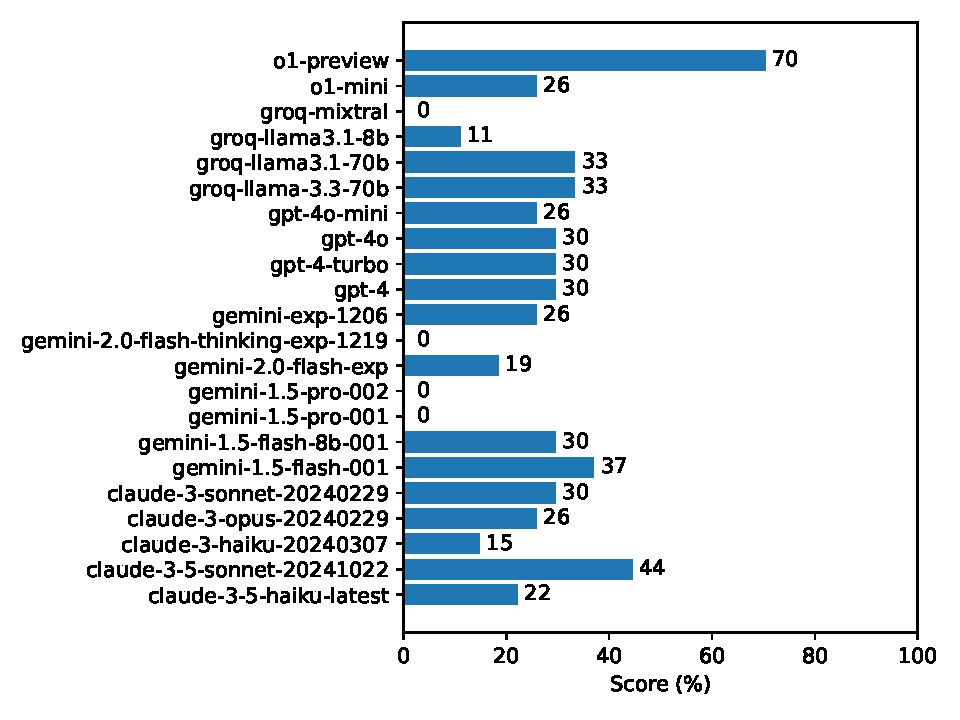
\includegraphics{llm_scores}
\end{document}